\documentclass[../main.tex]{subfiles}
\begin{document}

Chương này trình bày chi tiết phương pháp luận cốt lõi của đồ án: thiết kế Khung đo lường Behavioral Blending Score (BBS). Trước tiên, chương khảo sát sự thất bại của các bộ phát hiện truyền thống dưới góc nhìn toán học, từ đó xây dựng các công thức đo lường chính xác mức độ ngụy trang. Tiếp đến, luồng xử lý (pipeline) của hệ thống được thiết kế hoàn chỉnh. Cuối cùng, môi trường thử nghiệm thực tế được định nghĩa thông qua không gian đặc trưng V10, các kịch bản tạo sinh dữ liệu và mô hình SRAH.

\section{Khảo sát thực tế: Lý giải sự thất bại của UAD dưới góc nhìn toán học}
\label{section:2.1}

Sự sụp đổ của các mô hình Học máy không giám sát (UAD) trước các cuộc tấn công ngụy trang (LotL) không phải do cấu hình tham số, mà bắt nguồn từ những điểm mù toán học trong cấu trúc thuật toán.

\subsection{Sự thất bại của độ chồng lấn biên (Marginal Overlap)}
Trong nhiều nghiên cứu thực nghiệm, sự chồng lấn ở các phân phối biên đơn chiều thường được sử dụng làm cơ sở để đo lường độ khó của dữ liệu. Chỉ số tiêu biểu là **DDO (Degree of Distribution Overlap)**:
\begin{equation}
    DDO = \frac{1}{d} \sum_{s=1}^{d} \int \min\left( f_{a,s}(x_s),\ f_{b,s}(x_s) \right) dx_s
\end{equation}
Tuy nhiên, DDO giả định các đặc trưng hoạt động hoàn toàn độc lập với nhau. Trong thực tế, kẻ tấn công LotL ngụy trang để từng đặc trưng riêng lẻ trông hoàn toàn bình thường (DDO rất cao), nhưng sự kết hợp đồng thời của các đặc trưng đó lại là một sự kiện bất thường. Do đó, DDO không thể lý giải chính xác nguyên nhân thất bại của các thuật toán. Các thuật toán như iForest hay ECOD dựa trên chia cắt biên (Marginal Splits) đều bị vô hiệu hóa vì điểm mù này.

\subsection{Nghịch lý cấu trúc: Thiên kiến toàn cục và lỗ hổng cục bộ}
Để khắc phục điểm mù biên, các phương pháp không gian (như khoảng cách Mahalanobis) được đề xuất để đo lường toàn cục. Tuy nhiên, điều này dẫn đến một nghịch lý toán học: **Nghịch lý cấu trúc giữa Thiên kiến trung tâm toàn cục (Global Center Bias) và Lỗ hổng cục bộ (Local Pockets)**.

Một tiến trình độc hại có thể chui sâu vào trung tâm dữ liệu lành tính (có độ sâu Mahalanobis lớn, được hệ thống coi là an toàn tuyệt đối). Tuy nhiên, nếu xét bằng ước lượng mật độ nhân phi tham số (Kernel Density Estimation - KDE) để quan sát chi tiết cấu trúc cục bộ, tiến trình đó lại nằm trong một vùng không gian cực kỳ thưa thớt (Local Pocket) — nơi gần như không có tiến trình lành tính nào hoạt động. Sự thâm nhập này tạo ra thiên kiến toàn cục, khiến các mô hình học máy bị qua mặt hoàn toàn bởi xấp xỉ phân phối.

\section{Xây dựng khung đo lường toán học}
\label{section:2.2}

Dựa trên các khảo sát toán học, khung đo lường **Behavioral Blending Score (BBS)** được thiết kế nhằm lượng hóa chính xác độ sâu toàn cục của mã độc ngụy trang.

\subsection{Hiện tượng hòa trộn và khoảng cách Mahalanobis}
\begin{figure}[H]
\centering
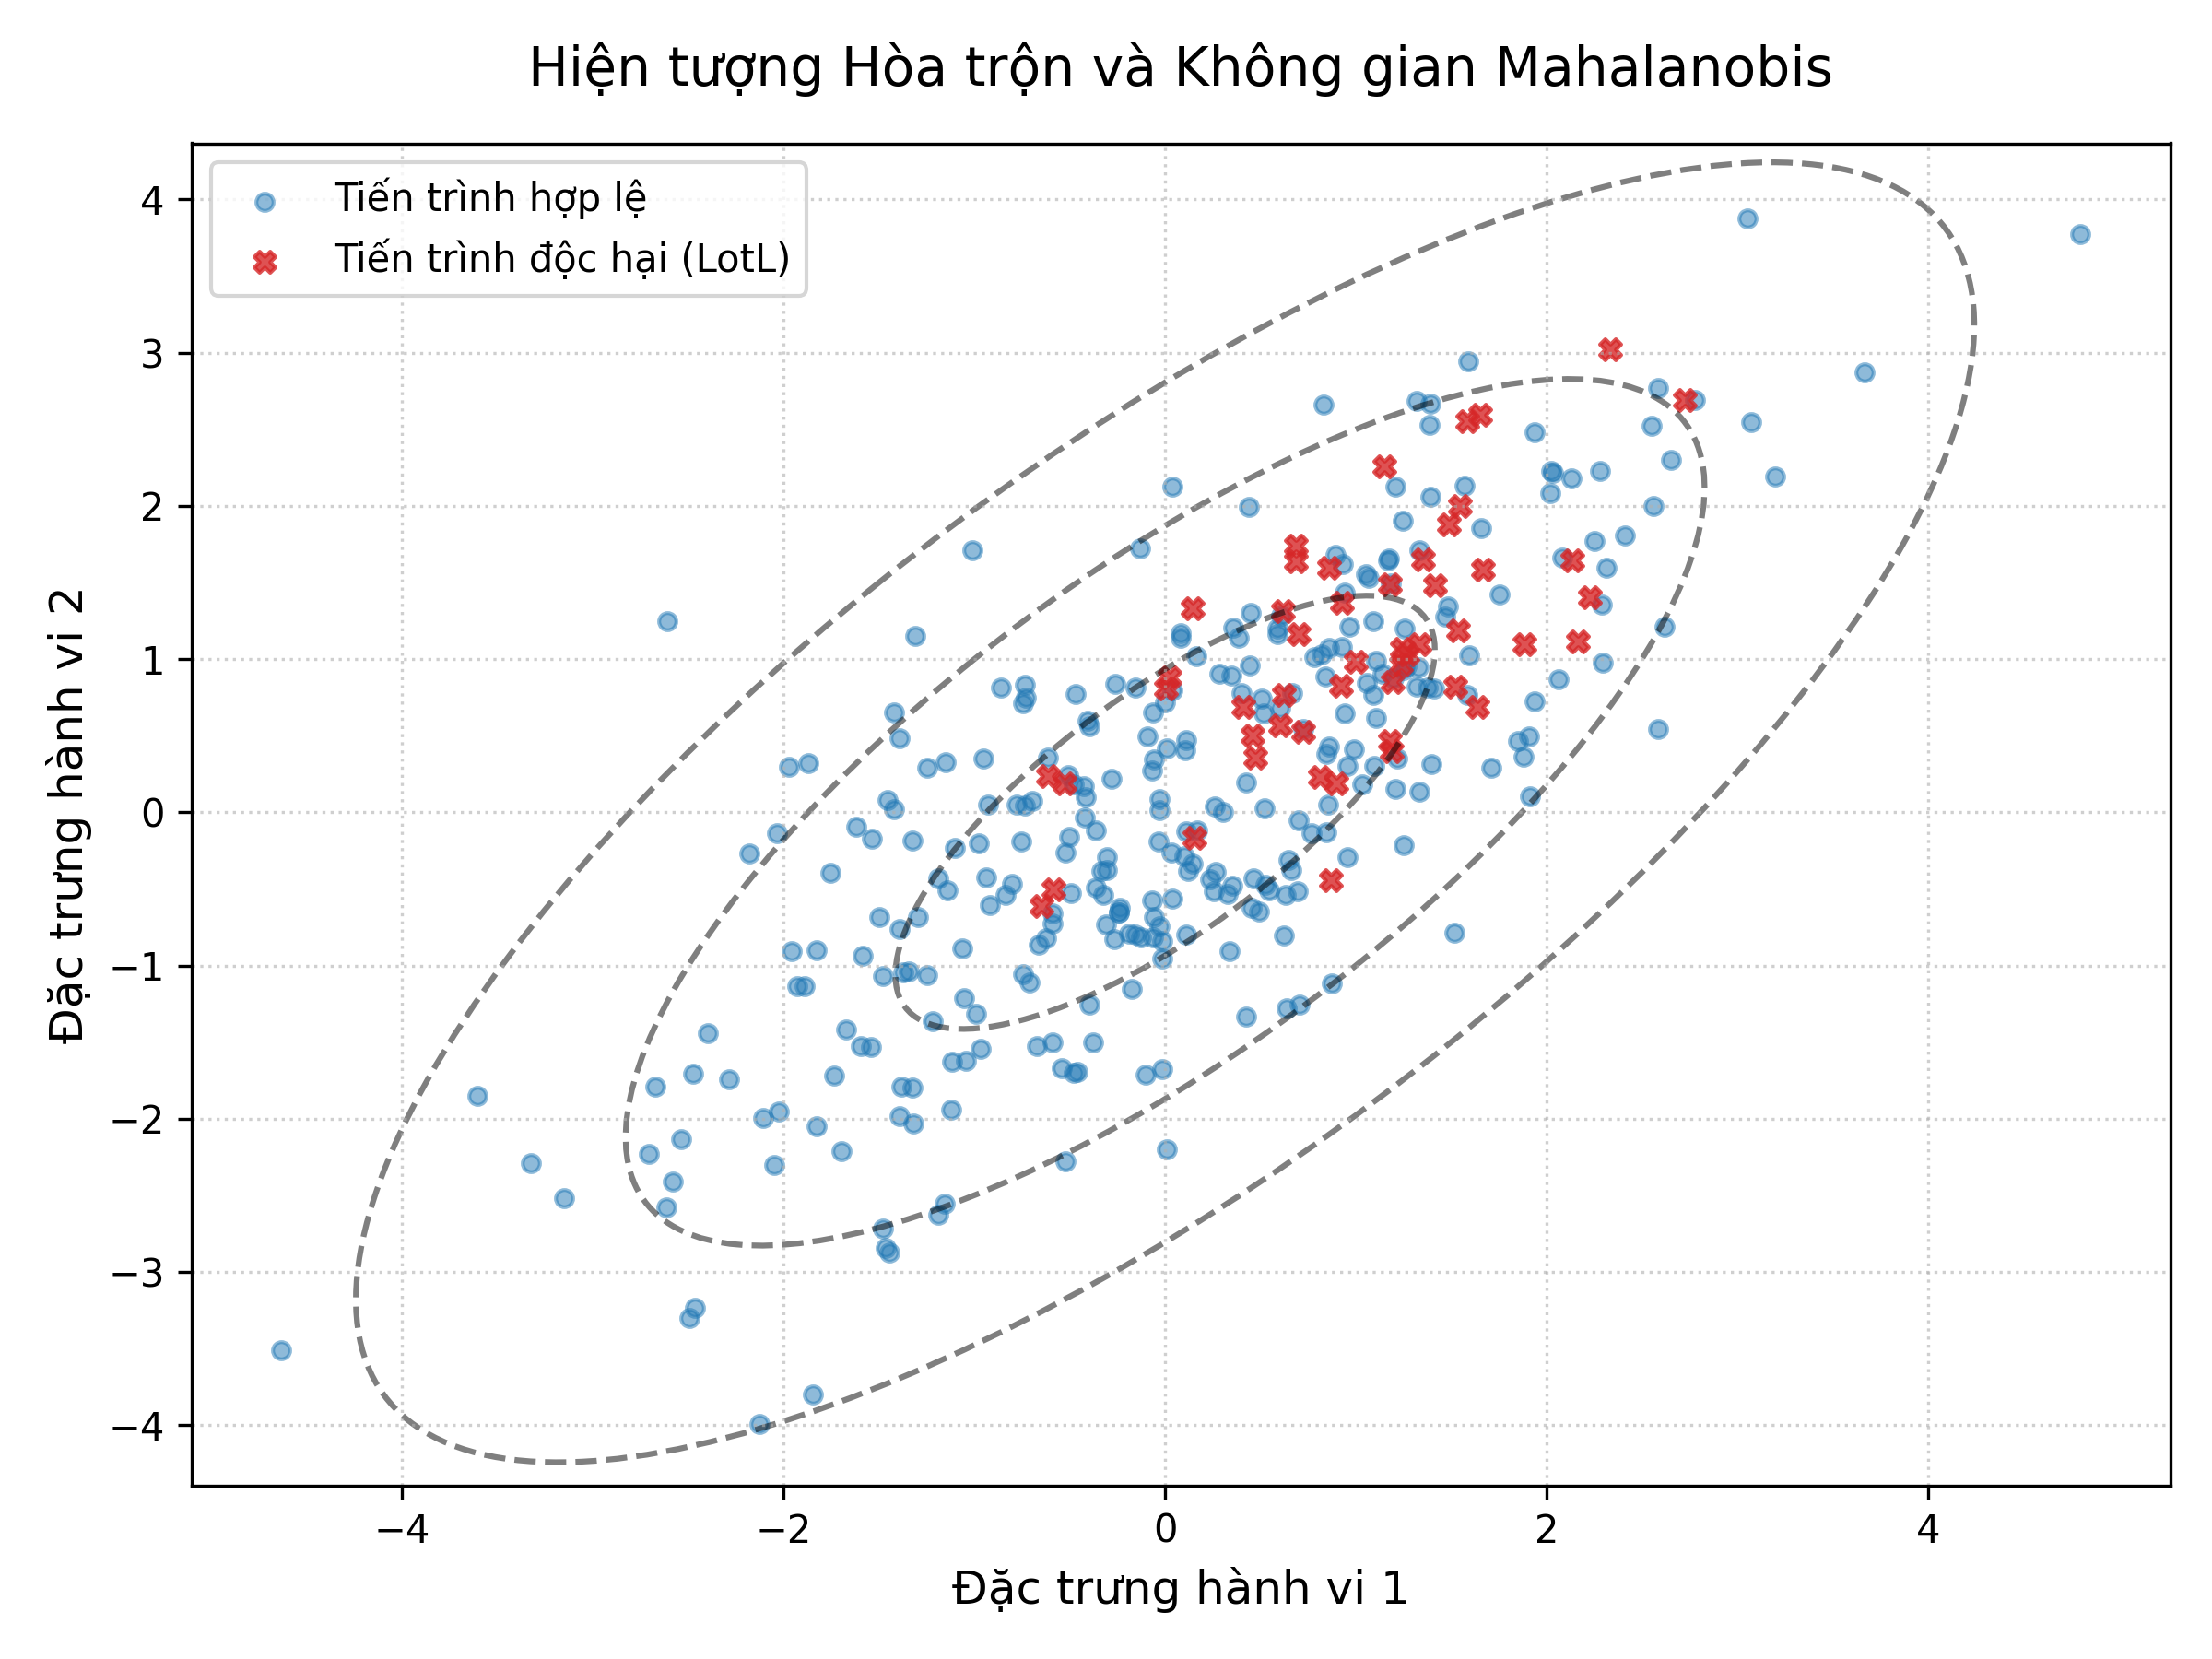
\includegraphics[width=0.8\textwidth]{../images/blending_mahalanobis.png}
\caption{Mô phỏng toán học hiện tượng Hòa trộn (Blending) và khoảng cách Mahalanobis.}
\label{fig:blending_mahalanobis}
\end{figure}

Khoảng cách Mahalanobis của một vector đặc trưng $x$ đối với phân phối nền (lành tính) được tính bằng:
\begin{equation}
    D_M(x) = \sqrt{(x - \mu)^T \Sigma^{-1} (x - \mu)}
\end{equation}
Trong đó $\mu$ là vector trung bình và $\Sigma$ là ma trận hiệp phương sai. Hình \ref{fig:blending_mahalanobis} mô phỏng cách mã độc ngụy trang lọt sâu vào các vòng elip hiệp phương sai, hòa trộn hoàn toàn vào dữ liệu bình thường.

\subsection{Thước đo cốt lõi DensPct\_Mahal}
Để chuyển đổi khoảng cách Mahalanobis thành một hàm mật độ (probability density), đồ án định nghĩa hàm $f_{Mahal}(x)$ dựa trên phân phối Gaussian đa chiều. Giả sử $F_b(t)$ là hàm phân phối tích lũy (CDF) của mật độ dữ liệu lành tính, thước đo độ sâu toàn cục DensPct\_Mahal cho tập dữ liệu độc hại $X_a$ được xác định:
\begin{equation}
    DensPct\_Mahal = \text{Median} \left[ F_b(f_{Mahal}(X_a)) \right]
\end{equation}
Chỉ số DensPct\_Mahal lượng hóa tỷ lệ phần trăm dữ liệu bình thường có mật độ thấp hơn hoặc bằng trung vị của dữ liệu tấn công. Giá trị này đóng vai trò là điểm neo hiệu chỉnh (Threshold Calibration) tương đương với Tỷ lệ báo động giả tại mức độ nhạy 50\% ($FPR@TPR_{0.5}$) của các hệ thống dựa trên khoảng cách.

\section{Thiết kế luồng xử lý (Pipeline) đo lường}
\label{section:2.3}

Để triển khai các công thức toán học vào thực tiễn, một luồng xử lý hệ thống (Pipeline) được thiết kế khép kín từ khâu thu thập dữ liệu thô đến khi trích xuất điểm số đo lường. Sơ đồ kiến trúc tổng thể được thể hiện trong Hình \ref{fig:bbs_pipeline}.

\begin{figure}[H]
\centering
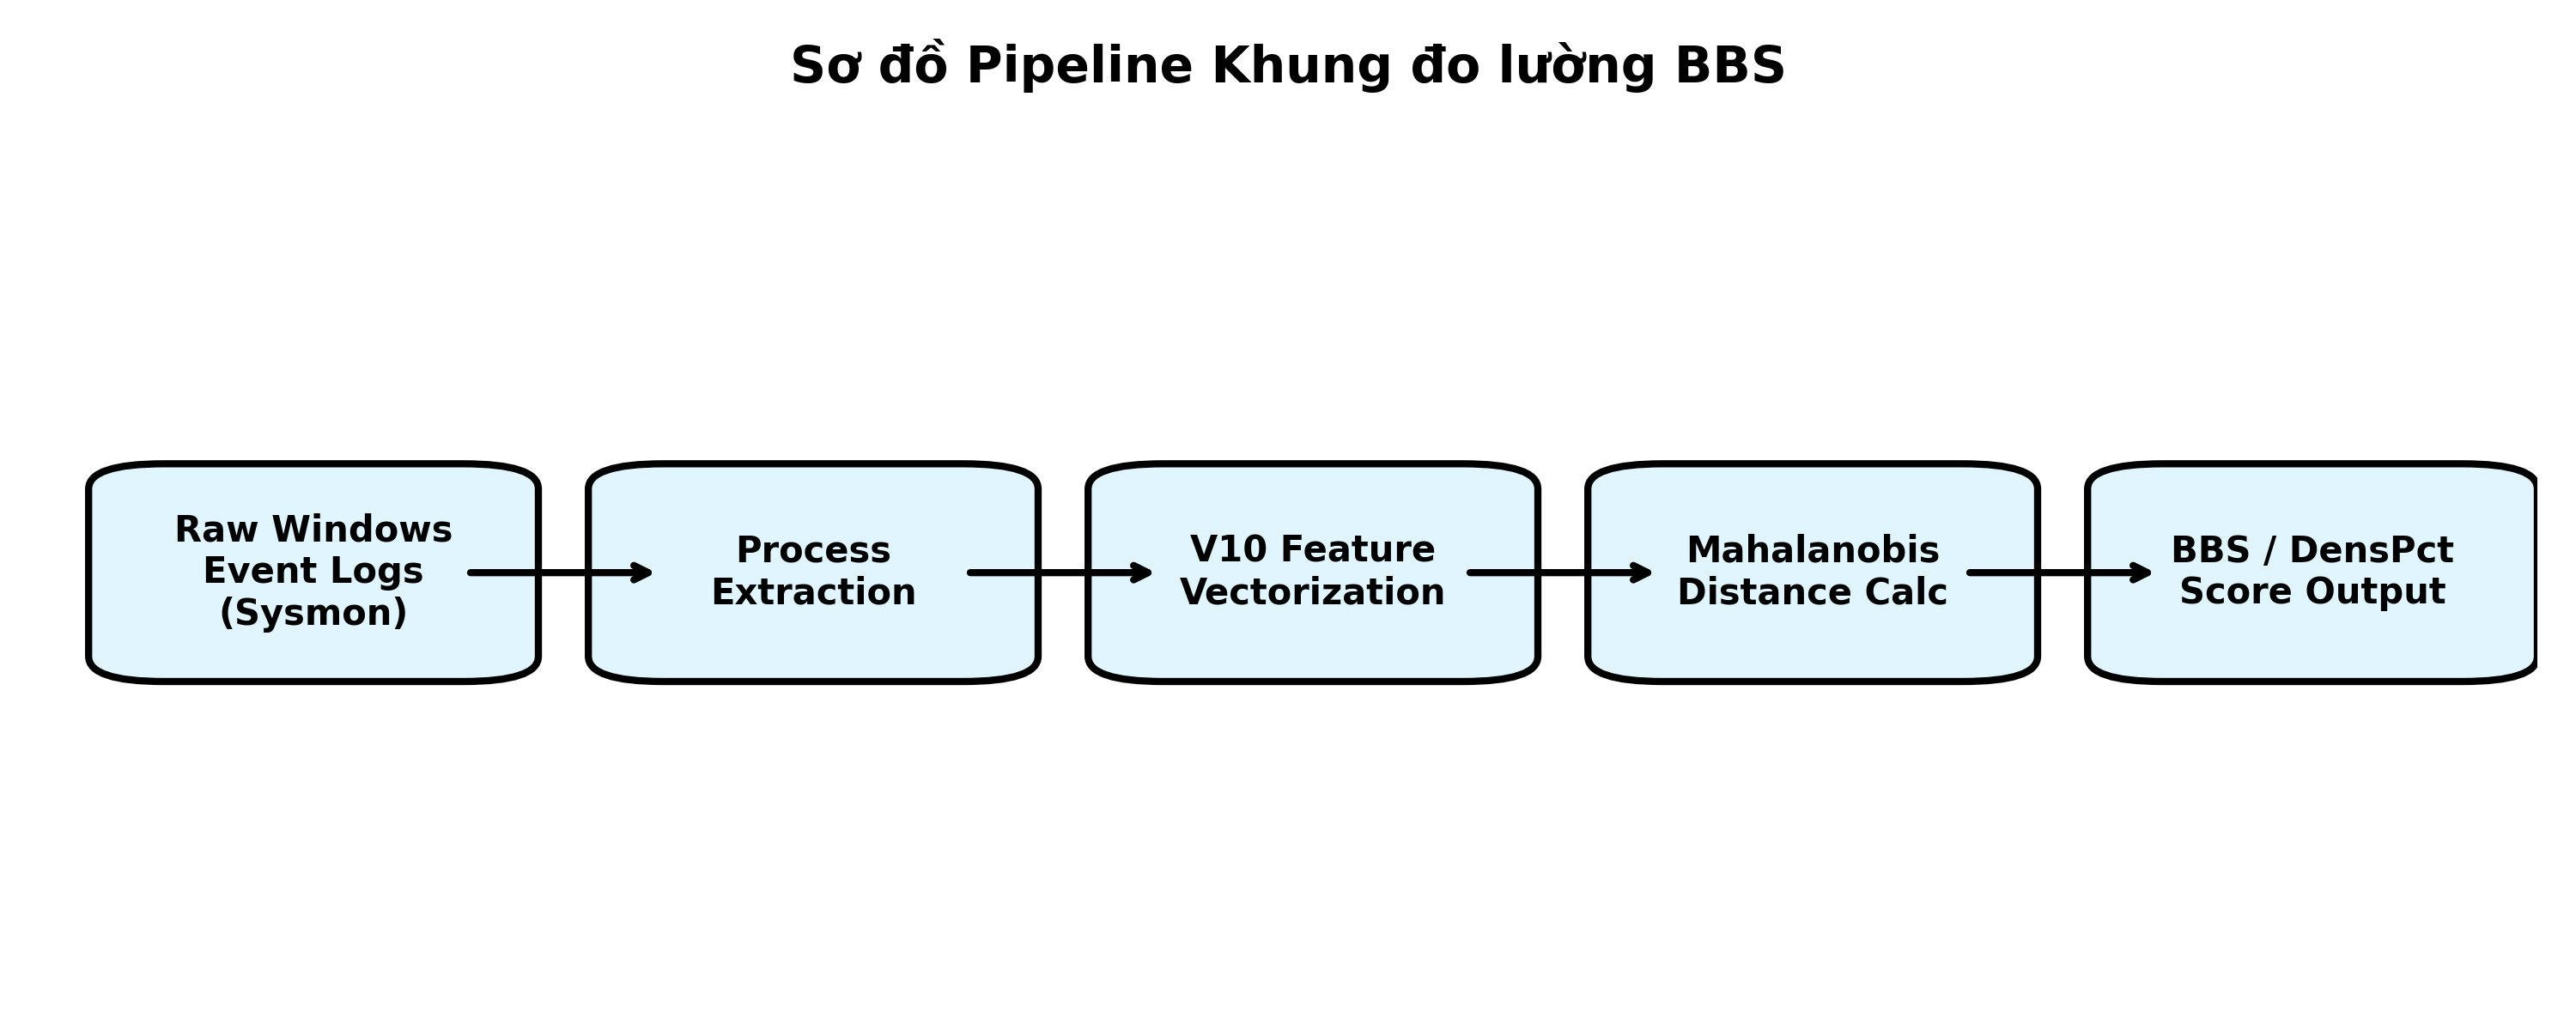
\includegraphics[width=\textwidth]{../images/bbs_pipeline.png}
\caption{Sơ đồ luồng xử lý (Pipeline) của Khung đo lường BBS.}
\label{fig:bbs_pipeline}
\end{figure}

Luồng xử lý bao gồm các giai đoạn:
1. **Raw Windows Event Logs:** Thu thập và phân tích cú pháp tệp `.evtx` của Sysmon.
2. **Process Extraction:** Tái tạo đồ thị tiến trình có hướng dựa trên ProcessGuid để giải quyết vấn đề PID tái sử dụng.
3. **V10 Feature Vectorization:** Biến đổi các hoạt động hành vi thành vector đặc trưng đa chiều hỗn hợp.
4. **Mahalanobis Distance Calc:** Thực thi tính toán ma trận hiệp phương sai nghịch đảo và đo lường khoảng cách toàn cục.
5. **BBS Score Output:** Tính toán CDF thực nghiệm và xuất ra điểm số DensPct\_Mahal để đánh giá độ khó.

\section{Thiết kế môi trường thử nghiệm}
\label{section:2.4}

Khung đo lường lý thuyết cần được triển khai và kiểm chứng trên một môi trường dữ liệu thực tiễn và khắt khe.

\subsection{Đề xuất Không gian đặc trưng hành vi V10}
Không gian đặc trưng hành vi hỗn hợp 10 chiều ($V_{10}$) được thiết kế nhằm bao phủ toàn bộ khía cạnh hoạt động: nội tại tiến trình (spatial), phả hệ thực thi (sequential), và giao tiếp mạng (collective).
Vector đặc trưng được định nghĩa: $V_{10} = [v_1, v_2, ..., v_{10}]$, tuân theo cấu hình kiểu dữ liệu hỗn hợp \texttt{uuuuccooou} (u: nhị phân, c: liên tục, o: thứ tự):

\begin{table}[H]
\centering
\small
\setlength{\tabcolsep}{4pt}
\caption{Ma trận không gian đặc trưng hành vi $V_{10}$ (cấu hình hỗn hợp \texttt{uuuuccooou}).}
\begin{tabular}{|>{\centering\arraybackslash}p{1.0cm}|p{4.0cm}|p{1.8cm}|p{1.8cm}|p{4.6cm}|}
\hline
\textbf{Ký hiệu} & \textbf{Tên Đặc trưng} & \textbf{Kiểu} & \textbf{Nguồn EID} & \textbf{Ý nghĩa Hành vi} \\ \hline
$v_1$ & \texttt{has\_network} & u (Binary) & EID 3 & Tiến trình sinh kết nối mạng \\ \hline
$v_2$ & \texttt{has\_injection} & u (Binary) & EID 8 & Có hành vi bơm mã (CreateRemoteThread) \\ \hline
$v_3$ & \texttt{has\_file\_drop} & u (Binary) & EID 11 & Ghi nhận tạo file mới trên đĩa cứng \\ \hline
$v_4$ & \texttt{has\_reg\_mod} & u (Binary) & EID 13 & Thay đổi registry để thiết lập duy trì \\ \hline
$v_5$ & \texttt{nif\_binary} & c (Continuous) & EID 1 & Độ hiếm của tên tiến trình nền \\ \hline
$v_6$ & \texttt{nif\_pair} & c (Continuous) & EID 1 & Độ hiếm của quan hệ cha - con \\ \hline
$v_7$ & \texttt{entropy\_bin} & o (Ordinal) & EID 1 & Entropy dòng lệnh (ngụy trang/mã hóa) \\ \hline
$v_8$ & \texttt{cmd\_len\_bin} & o (Ordinal) & EID 1 & Độ dài dòng lệnh phân theo khoảng \\ \hline
$v_9$ & \texttt{child\_count\_bin} & o (Ordinal) & EID 1 & Số lượng tiến trình con được khởi tạo \\ \hline
$v_{10}$ & \texttt{parent\_sigma\_bin} & u (Binary) & EID 1 & Cha bị phát hiện bởi luật tĩnh Sigma \\ \hline
\end{tabular}
\label{tab:v10_space}
\end{table}

\subsection{Cơ chế bơm dữ liệu có kiểm soát (Controlled Injection)}
Để tạo ra các kịch bản đo lường đa dạng, cơ chế **Controlled Injection** được triển khai. Cơ chế này lấy một tập log lành tính làm môi trường nền (\textit{benign baseline}), sau đó bơm trực tiếp các tiến trình tấn công mô phỏng (khoảng $20 \sim 50$ tiến trình) với tỷ lệ cực thấp ($\ll 0.1\%$). Tám tập dữ liệu tổng hợp (từ KB1 đến KB8) được chế tác để mô phỏng chính xác các kỹ thuật MITRE ATT\&CK với mức độ ngụy trang tăng dần (từ việc gọi macro đơn giản đến di chuyển ngang không tập tin).

\subsection{Kịch bản thử nghiệm các mô hình UAD}
Để kiểm chứng hiệu quả của khung đo lường BBS trong việc dự đoán sự sụp đổ của AI, các tập dữ liệu sẽ được đưa qua 4 mô hình phát hiện:
\begin{itemize}
    \item \textbf{iForest \& ECOD}: Các mô hình truyền thống đại diện cho thiên kiến phân phối biên (Marginal Splits).
    \item \textbf{SRAH}: Mô hình tích hợp đa cảm biến biên (Multi-sensor UAD), dùng để đối chiếu khả năng khắc phục điểm mù.
    \item \textbf{KDE\_Joint}: Mô hình đề xuất sử dụng ước lượng mật độ nhân đồng thời (Mixed Product KDE) phi tham số. Mô hình này hoạt động như một bằng chứng tồn tại (Existence Proof) để khẳng định mã độc ngụy trang có thể bị bóc trần nếu khai thác đúng các lỗ hổng mật độ cục bộ (Local Pockets).
\end{itemize}

\end{document}
